\section{Methodology}
\label{sec:method}
\subsection{Task and Source Boundaries}
Each inference unit receives a dataset-supplied entry title, a public advisory description truncated at 1,500 characters, a repository URL, and a pinned vulnerable commit. It returns at most five repository-relative paths with line intervals and brief reasons. The title comes from the entry-level \texttt{vuln\_title} field, whose schema permits annotators to append a filename to distinguish entries~\cite{vulngymdata}. It is not necessarily the original public advisory title. Explicit EP/CO paths and intervals enter evaluation only; filename information can also enter inference through the supplied title. All configurations receive the same title and description at final inference. Agent and RAG use them during acquisition; Pack's acquisition is task-independent.

Let $U$ denote files authorized before acquisition, $S$ the source spans delivered during a unit, and $T$ the unique EP/CO target files. Write $F(S)$ for the file-path projection of those spans. A listing exposes paths but contributes no code spans to $S$. Thus $T\cap U$ concerns eligibility, whereas $|T\cap F(S)|/|T|$ measures target-file source delivery. A hit means that some source from that file reached the model; it does not establish that the annotated lines were delivered or used.

S1 materializes a content-hashed manifest for each canonical repository--commit snapshot. It admits a frozen source-extension list and extensionless text files; excludes symlinks, specified dependency/generated directories, files above 200,000 bytes, and files with a NUL byte in the first 8,192 bytes; and normalizes newlines. Each manifest binds authorized content to its pinned Git blob. Tools, packing, and retrieval construction use these manifests.

The common authorized universe contains 439,166 files across 74 snapshots. Of these, 832 are empty or entirely whitespace and produce no RAG chunks. RAG's actual indexed universe is therefore 438,334 files. Every nonblank eligible file is available to all three configurations, including all 130 entry-specific EP/CO target files and 204 entry-specific trace files. File totals sum snapshots; the target totals deduplicate paths within each entry before summing entries.

\begin{figure*}[t]
\centering
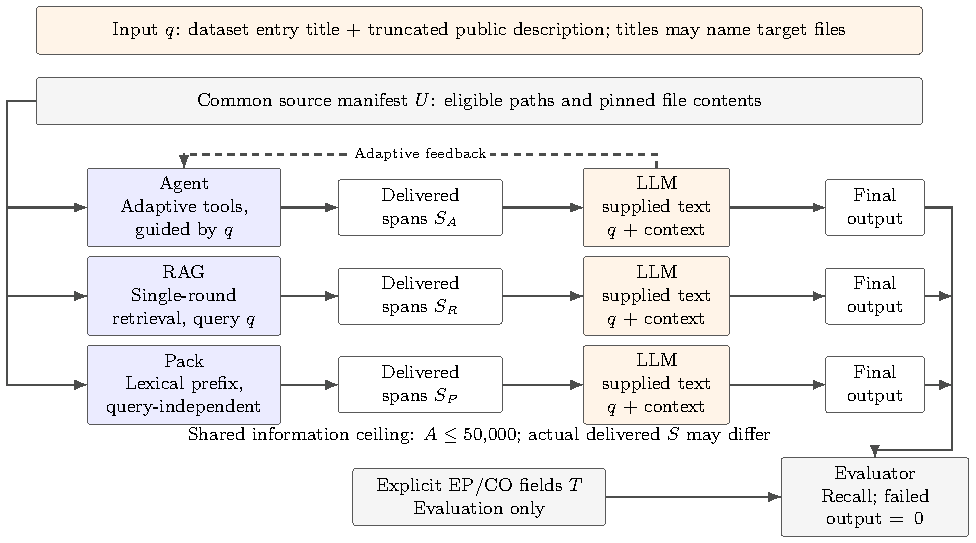
\includegraphics[width=0.94\textwidth]{figures/acquisition_design.pdf}
\caption{S1 acquisition and evaluation boundaries. The supplied entry title and public description guide Agent and RAG acquisition and enter final inference in every configuration. Explicit EP/CO fields $T$ enter evaluation only; entry titles may contain target filenames. Shared eligibility does not imply identical delivered source $S$ or valid final outputs.}
\label{fig:design}
\end{figure*}

\subsection{Acquisition Configurations}
\textbf{Pack.} Eligible relative paths are ordered lexicographically. A path list consumes at most 5,000 accounting tokens; numbered source lines are then appended in lexical file order within the remaining information budget. The renderer retains complete lines. This deterministic prefix is a low-complexity static reference, not a representative implementation of all context-packing strategies.

\textbf{RAG.} The dataset-supplied entry title and truncated public description form one retrieval query. Nonblank source is chunked into 60-line windows with 15-line overlap, without a chunk-count cap. BM25 uses lowercased alphanumeric/underscore terms. Dense retrieval uses BAAI/bge-small-en-v1.5~\cite{bge} through FastEmbed, cosine similarity, and a frozen 400-accounting-token truncation rule for chunk embedding text. The runtime ONNX and tokenizer bytes are hash-bound; its recorded ONNX snapshot is \texttt{aa8f8b0}, not asserted to be the upstream BAAI commit. The model-card sequence limit is 512 model tokens, a different tokenizer boundary from the chunk truncation rule. Query text is passed directly through \texttt{embed}, without an explicitly prepended retrieval instruction. Exact artifact hashes and current dependency behavior are indexed in Appendix~A. Reciprocal rank fusion~\cite{rrf} scores chunk $c$ as
\begin{equation}
 r(c)=\frac{1}{60+r_{\mathrm{sparse}}(c)}
      +\frac{1}{60+r_{\mathrm{dense}}(c)}.
\end{equation}
Complete sparse and dense rankings are fused; ties use sparse rank, relative path, and starting line. Selected chunks are rendered with headers and numbered lines until the ledger ceiling is reached. The model receives one acquisition pass, followed by final-answer handling.

\textbf{Agent.} Pi's native tool interface exposes only \texttt{list\_dir}, \texttt{grep}, and \texttt{read\_file}. Built-in general-purpose tools are disabled. Listings return at most 200 children. Search uses POSIX extended regular expressions, an optional file glob, at most 50 matches, and two surrounding lines. Reads return at most 400 lines. Tool-output caps are 4,000 accounting tokens for listings/search and 8,000 for reads. Search and read operations authorize paths against the manifest. The model chooses actions from the advisory and earlier results; the native loop may issue multiple calls in one assistant message.

At most 40 accepted bridge execution actions and 46 provider requests are permitted per unit. The action limit does not count every model tool attempt: Pi may reject arguments before bridge execution. Agent's stateful interaction also differs from the single context presentation used by Pack and RAG.

\subsection{Final-Answer Handling and Termination}
S1 validates the defined JSON/XML-compatible answer envelope, including positive integer line coordinates. Nonempty invalid final text receives at most one formatting correction requesting only the final JSON object. Empty final text fails directly without that correction. The native collector retains text from the last completed assistant message, excludes thinking blocks from answers, and finishes after the native loop settles. DSML tool-call text is outside the accepted final-answer forms.

When a normal bridge action reaches the action or information ceiling, the extension disables active tools. That action still returns its source or listing text plus an exhaustion flag stored in tool-result details. It does not append a new final-answer instruction at that transition. The bridge returns an explicit budget-exhausted instruction if another queued call starts with the budget already exhausted. An offline probe of the installed Pi message converter shows that tool-result details are not sent as model-visible content. Initial instructions and any later formatting correction remain distinct from this transition.

The transport has a 600-second completion-wait timeout, initially measured from prompt start and reset at each completed assistant message. It is not a 600-second total task limit and is not reset at each token. S0 instead applies a 600-second timeout to each explicit prompt. No retained effective unit exceeds 600 seconds in recorded total time (maxima: S0 531.2 seconds, S1 387.0 seconds). Interrupted infrastructure attempts are recorded separately.

\subsection{Information and Resource Accounting}
The shared repository-information ceiling is $A\leq50{,}000$. $A$ sums newly delivered blocks using \texttt{cl100k\_base}: source headers, numbered code, listings, search results, repeated acquisitions, and errors represented in the bridge ledger. Replayed conversation history is not charged again to $A$. Exact block text, token counts, hashes, and source spans are recorded.

This is a ledger of acquisition output, not all model-visible feedback. S1 contains 174 Pi argument-validation error results (173 search, one read) that bypass the bridge and enter neither $A$ nor its execution-action count. They deliver no new repository source. Consequently, the verified ceiling bounds the ledger and delivered repository content; it does not assert that every feedback token is included.

We separately measure cumulative provider input $B$, output tokens, provider-reported fees, and recorded unit time. $B$ includes instructions, advisory text, delivered blocks, replayed history, and cached input. Its tokenizer and scope differ from $A$; the two counts must not be treated as interchangeable budgets. Offline source preparation and index construction are excluded from online timing. The recorded unit window begins after initial source/index validation and some model preparation, so it is not full cold-start latency.
